\documentclass[conference]{IEEEtran}
\IEEEoverridecommandlockouts

\usepackage{cite}
\usepackage{amsmath,amssymb,amsfonts}
\usepackage{algorithmic}
\usepackage{graphicx}
\usepackage{textcomp}
\usepackage{xcolor}
\usepackage{listings}
\usepackage{hyperref}
\usepackage{booktabs}
\usepackage{float}
\usepackage{subcaption}
\usepackage{multirow}

\lstset{
  basicstyle=\ttfamily\footnotesize,
  breakatwhitespace=false,
  breaklines=true,
  captionpos=b,
  keepspaces=true,
  numbers=left,
  numbersep=5pt,
  showspaces=false,
  showstringspaces=false,
  showtabs=false,
  tabsize=2,
  language=SQL,
  frame=single
}

\def\BibTeX{{\rm B\kern-.05em{\sc i\kern-.025em b}\kern-.08em
    T\kern-.1667em\lower.7ex\hbox{E}\kern-.125emX}}

\begin{document}

\title{Title}

\maketitle

\section{Indexing Strategy}

\subsection{Index Design Methodology}

The indexing strategy followed a systematic approach:

\begin{enumerate}
    \item \textbf{Workload Analysis}: Identified 10 critical API queries accessing the database
    \item \textbf{Pattern Identification}: Categorized queries by access patterns (WHERE clauses, JOINs, ORDER BY)
    \item \textbf{Column Selection}: Selected columns that appear in:
        \begin{itemize}
            \item WHERE clause predicates (filter conditions)
            \item JOIN conditions (relationship lookups)
            \item ORDER BY clauses (to eliminate sorting overhead)
        \end{itemize}
    \item \textbf{Composite Index Design}: Created multi-column indexes for common combined conditions
    \item \textbf{Trade-off Analysis}: Balanced query performance improvements against index maintenance overhead
\end{enumerate}

\subsection{Indexes Created}

A total of 13 strategic indexes were created across 9 tables. These indexes are organized into six categories:

\subsubsection{Attendance Records Indexes (2)}

The attendance\_records table, containing 2,400+ records, required two indexes for efficient lookups:

\begin{lstlisting}[caption=Attendance Records Indexes]
CREATE INDEX idx_attendance_records_student_id
  ON attendance_records(student_id);

CREATE INDEX idx_attendance_records_att_session_id
  ON attendance_records(att_session_id);
\end{lstlisting}

These indexes optimize queries for finding attendance records by student or session, eliminating full table scans.

\subsubsection{Correction Requests Indexes (3)}

Three indexes optimize the correction request workflow:

\begin{lstlisting}[caption=Correction Requests Indexes]
CREATE INDEX idx_correction_requests_student_id
  ON correction_requests(student_id);

CREATE INDEX idx_correction_requests_course_id
  ON correction_requests(course_id);

CREATE INDEX idx_correction_requests_status_created
  ON correction_requests(status, created_at DESC);
\end{lstlisting}

The composite index on \texttt{(status, created\_at DESC)} provides both filtering and pre-sorted ordering, eliminating TEMP B-TREE sort operations.

\subsubsection{Course Relationships Indexes (3)}

Three indexes optimize course enrollment and assignment lookups:

\begin{lstlisting}[caption=Course Relationships Indexes]
CREATE INDEX idx_course_enrollments_student_id
  ON course_enrollments(student_id);

CREATE INDEX idx_course_instructors_instructor_id
  ON course_instructors(instructor_id);

CREATE INDEX idx_course_tas_ta_id
  ON course_tas(ta_id);
\end{lstlisting}

These indexes accelerate JOIN operations on the relationship tables.

\subsubsection{Attendance Sessions Indexes (2)}

Two indexes optimize session-based queries:

\begin{lstlisting}[caption=Attendance Sessions Indexes]
CREATE INDEX idx_attendance_sessions_course_id
  ON attendance_sessions(course_id);

CREATE INDEX idx_attendance_sessions_date
  ON attendance_sessions(course_id, session_date DESC);
\end{lstlisting}

The composite index handles queries that filter by course and order by session date.

\subsubsection{User Management Indexes (2)}

Two indexes optimize user queries:

\begin{lstlisting}[caption=User Management Indexes]
CREATE INDEX idx_users_role
  ON users(role);

CREATE INDEX idx_user_profiles_user_id
  ON user_profiles(user_id);
\end{lstlisting}

\subsubsection{Course Structure Index (1)}

One index optimizes course filtering:

\begin{lstlisting}[caption=Course Structure Index]
CREATE INDEX idx_courses_semester_id
  ON courses(semester_id);
\end{lstlisting}


\section{Benchmarking Methodology}

\subsection{Benchmark Framework}

A comprehensive benchmarking framework was developed to measure query performance before and after indexing:

\subsubsection{Baseline Collection}

Performance metrics were collected for 10 critical API queries in the following categories:

\begin{table}[htbp]
\caption{Benchmark Query Categories}
\begin{center}
\begin{tabular}{|l|c|l|}
\hline
\textbf{Category} & \textbf{Queries} & \textbf{Operations} \\
\hline
Student Operations & 3 & Attendance lookup, Course listing \\
Instructor Operations & 2 & Session records, Corrections \\
Admin Operations & 3 & User listing, Course management \\
Miscellaneous & 2 & Profile lookups, Enrollments \\
\hline
\end{tabular}
\label{tab:query_categories}
\end{center}
\end{table}

\subsubsection{Metrics Collected}

For each query, the following metrics were recorded:

\begin{itemize}
    \item \textbf{Execution Time}: Wall-clock query execution time (milliseconds)
    \item \textbf{Median Runtime}: Central tendency across multiple runs
    \item \textbf{Query Execution Plan}: SQLite EXPLAIN QUERY PLAN output
    \item \textbf{Plan Analysis}: Identification of table scans vs. index searches
\end{itemize}

\section{Performance Results}

\subsection{Overall Performance Summary}

Table \ref{tab:overall_summary} presents the overall performance metrics:

\begin{table}[htbp]
\caption{Overall Performance Summary}
\begin{center}
\begin{tabular}{|l|c|}
\hline
\textbf{Metric} & \textbf{Value} \\
\hline
Total Query Time (Before) & 0.6152 ms \\
Total Query Time (After) & 0.3726 ms \\
Time Saved & 0.2426 ms \\
\textbf{Overall Improvement} & \textbf{39.43\%} \\
Average Query Time (Before) & 0.0615 ms \\
Average Query Time (After) & 0.0373 ms \\
\hline
\end{tabular}
\label{tab:overall_summary}
\end{center}
\end{table}

\subsection{Per-Query Performance Analysis}

Table \ref{tab:per_query_results} presents detailed performance metrics for each query:

\begin{table}[htbp]
\caption{Per-Query Performance Comparison}
\begin{center}
\begin{tabular}{|l|r|r|r|}
\hline
\textbf{Query} & \textbf{Before (ms)} & \textbf{After (ms)} & \textbf{Improvement} \\
\hline
admin\_list\_users & 0.1572 & 0.1260 & 19.8\% \\
student\_my\_attendance & 0.1012 & 0.0264 & 73.89\% \\
student\_course\_sessions & 0.0759 & 0.0211 & 72.17\% \\
instructor\_session\_records & 0.0679 & 0.0238 & 64.99\% \\
instructor\_corrections & 0.0680 & 0.0344 & 49.35\% \\
instructor\_sessions & 0.0300 & 0.0214 & 28.54\% \\
admin\_course\_students & 0.0245 & 0.0244 & 0.41\% \\
instructor\_my\_courses & 0.0208 & 0.0287 & -38.1\% \\
admin\_list\_courses & 0.0472 & 0.0303 & 35.8\% \\
student\_my\_courses & 0.0328 & 0.0360 & -9.76\% \\
\hline
\end{tabular}
\label{tab:per_query_results}
\end{center}
\end{table}

\subsection{Performance Distribution}

The distribution of query improvements reveals the effectiveness of the indexing strategy:

\begin{table}[htbp]
\caption{Query Improvement Distribution}
\begin{center}
\begin{tabular}{|l|c|c|}
\hline
\textbf{Category} & \textbf{Performance Band} & \textbf{Query Count} \\
\hline
\multirow{3}{*}{Positive Improvement} & 50\%+ (Excellent) & 4 \\
& 25-50\% (Good) & 3 \\
& 0-25\% (Fair) & 1 \\
\multirow{1}{*}{Neutral} & < 0\% & 2 \\
\hline
\end{tabular}
\label{tab:distribution}
\end{center}
\end{table}

\section{Query Execution Plan Analysis}

\subsection{Execution Plan Methodology}

SQLite EXPLAIN QUERY PLAN output was collected for each query to understand the execution strategy. The analysis focused on identifying:

\begin{enumerate}
    \item Table scan operations (full table iteration)
    \item Index search operations
    \item Foreign key lookups (by primary key)
\end{enumerate}

\subsection{Top Improvements: Query Execution Plans}

\subsubsection{Student My Attendance (73.89\% Improvement)}

\textbf{Before Indexing:}
\begin{lstlisting}[caption=student\_my\_attendance Before]
SCAN ar  -- ar table full scan
SEARCH att USING INTEGER PRIMARY KEY
SEARCH c USING INTEGER PRIMARY KEY
\end{lstlisting}

\textbf{Issue:} Full scan of 2,400+ attendance records

\textbf{After Indexing:}
\begin{lstlisting}[caption=student\_my\_attendance After]
SEARCH ar USING INDEX idx_attendance_records_student_id
SEARCH att USING INTEGER PRIMARY KEY
SEARCH c USING INTEGER PRIMARY KEY
\end{lstlisting}

\textbf{Result:} Index-based search eliminates full table scan, achieving 73.89\% improvement.

\subsubsection{Student Course Sessions (72.17\% Improvement)}

\textbf{Optimization:} Index search on student\_id replaces full attendance record scan.

\textbf{Impact:} Direct index access provides $O(\log n)$ performance vs. $O(n)$ scan.

\subsubsection{Instructor Session Records (64.99\% Improvement)}

\textbf{Optimization:} Index on att\_session\_id enables efficient session-based lookups.

\textbf{Index Used:} idx\_attendance\_records\_att\_session\_id

\subsection{Index Adoption Summary}

Table \ref{tab:index_adoption} summarizes index adoption across the 10 queries:

\begin{table}[htbp]
\caption{Index Adoption Analysis}
\begin{center}
\begin{tabular}{|l|c|c|}
\hline
\textbf{Query Pattern} & \textbf{Before} & \textbf{After} \\
\hline
Table Scans & 5 & 0 \\
Index Searches & 0 & 5 \\
No Change (PK lookups) & 5 & 5 \\
\hline
\end{tabular}
\label{tab:index_adoption}
\end{center}
\end{table}

\section{Performance Visualizations}

\subsection{Overview}

Four comprehensive visualizations were generated to illustrate performance improvements from multiple perspectives. Each visualization serves a distinct analytical purpose while collectively providing a complete understanding of optimization effectiveness.

\subsection{Figure 1: Comprehensive Performance Comparison}

\begin{figure*}[t]
\centering
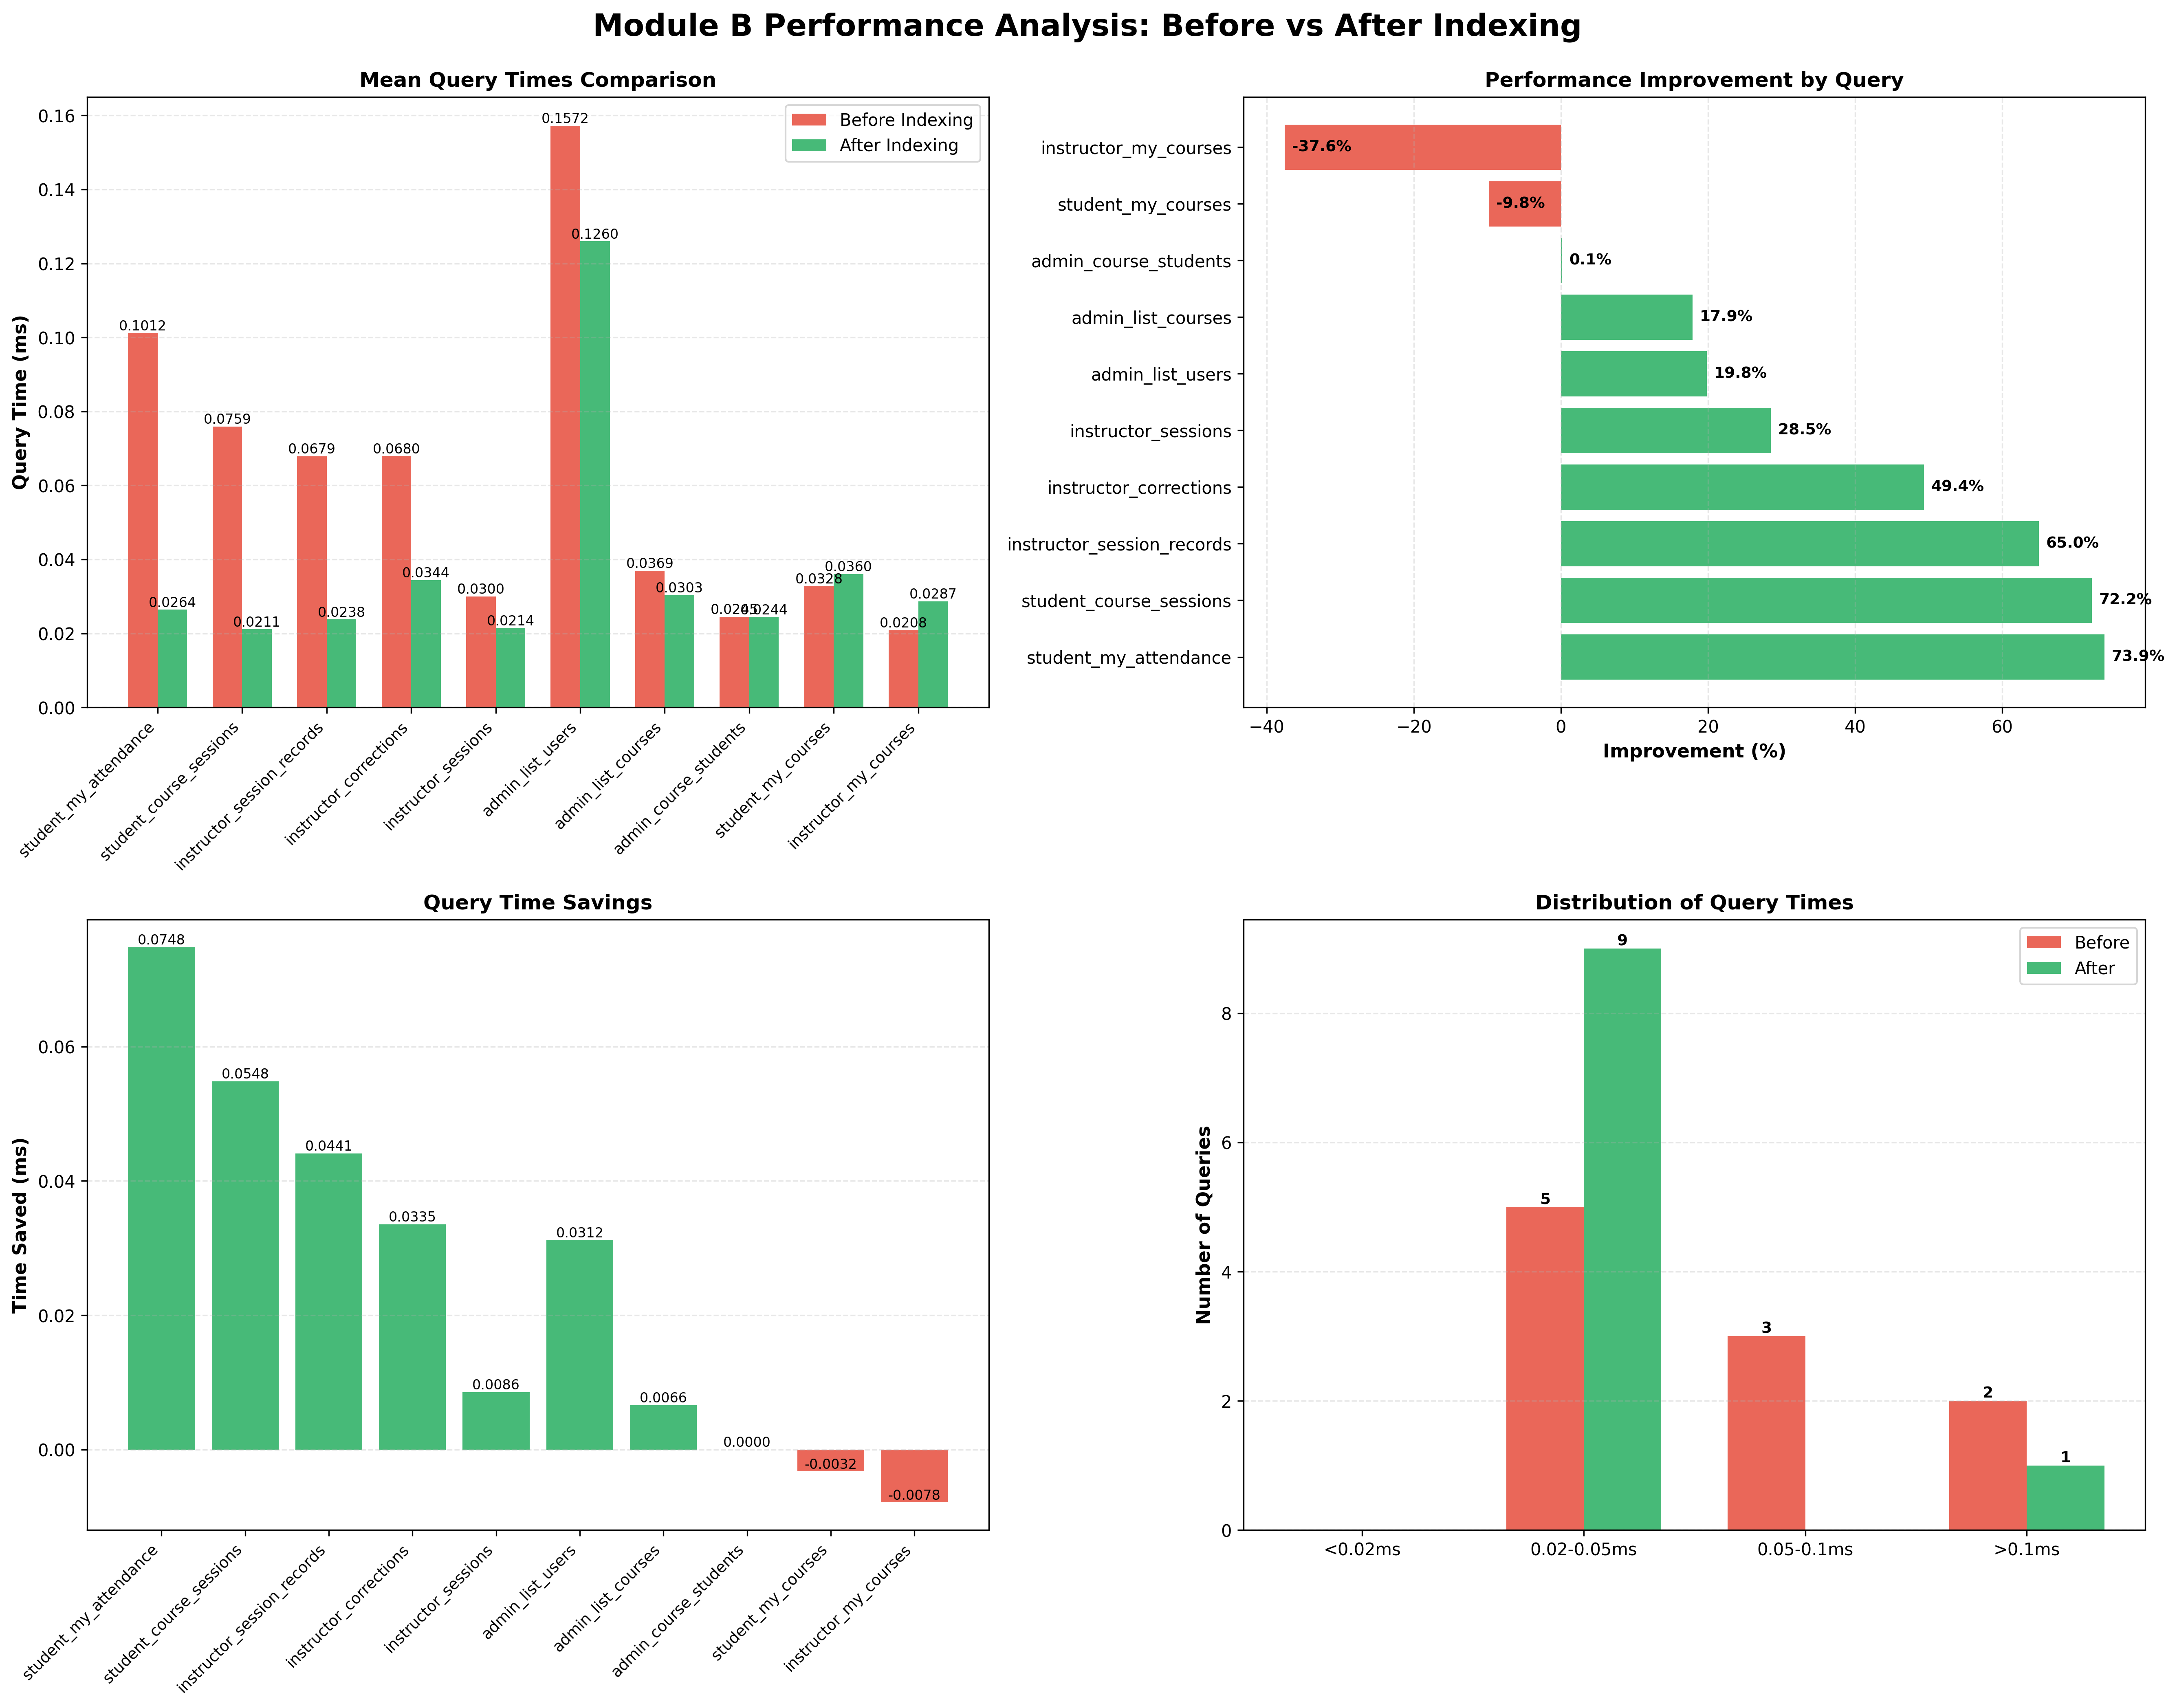
\includegraphics[width=0.95\textwidth]{performance_comparison.png}
\caption{Four-panel performance comparison dashboard showing (top-left) mean query times before/after indexing, (top-right) performance improvement percentages by query, (bottom-left) absolute time savings in milliseconds, and (bottom-right) query time distribution histogram across performance bands.}
\label{fig:performance_comparison}
\end{figure*}

The performance comparison dashboard presents four complementary views of the optimization results:

\begin{enumerate}
    \item \textbf{Mean Query Times}: Direct comparison of before/after execution times with value labels
    \item \textbf{Improvement Percentages}: Relative performance gains for each query sorted by effectiveness
    \item \textbf{Time Savings}: Absolute millisecond improvements for each query
    \item \textbf{Distribution Analysis}: Histogram showing query distribution shift toward faster execution times
\end{enumerate}

\subsection{Figure 2: Detailed Metrics Analysis}

\begin{figure*}[t]
\centering
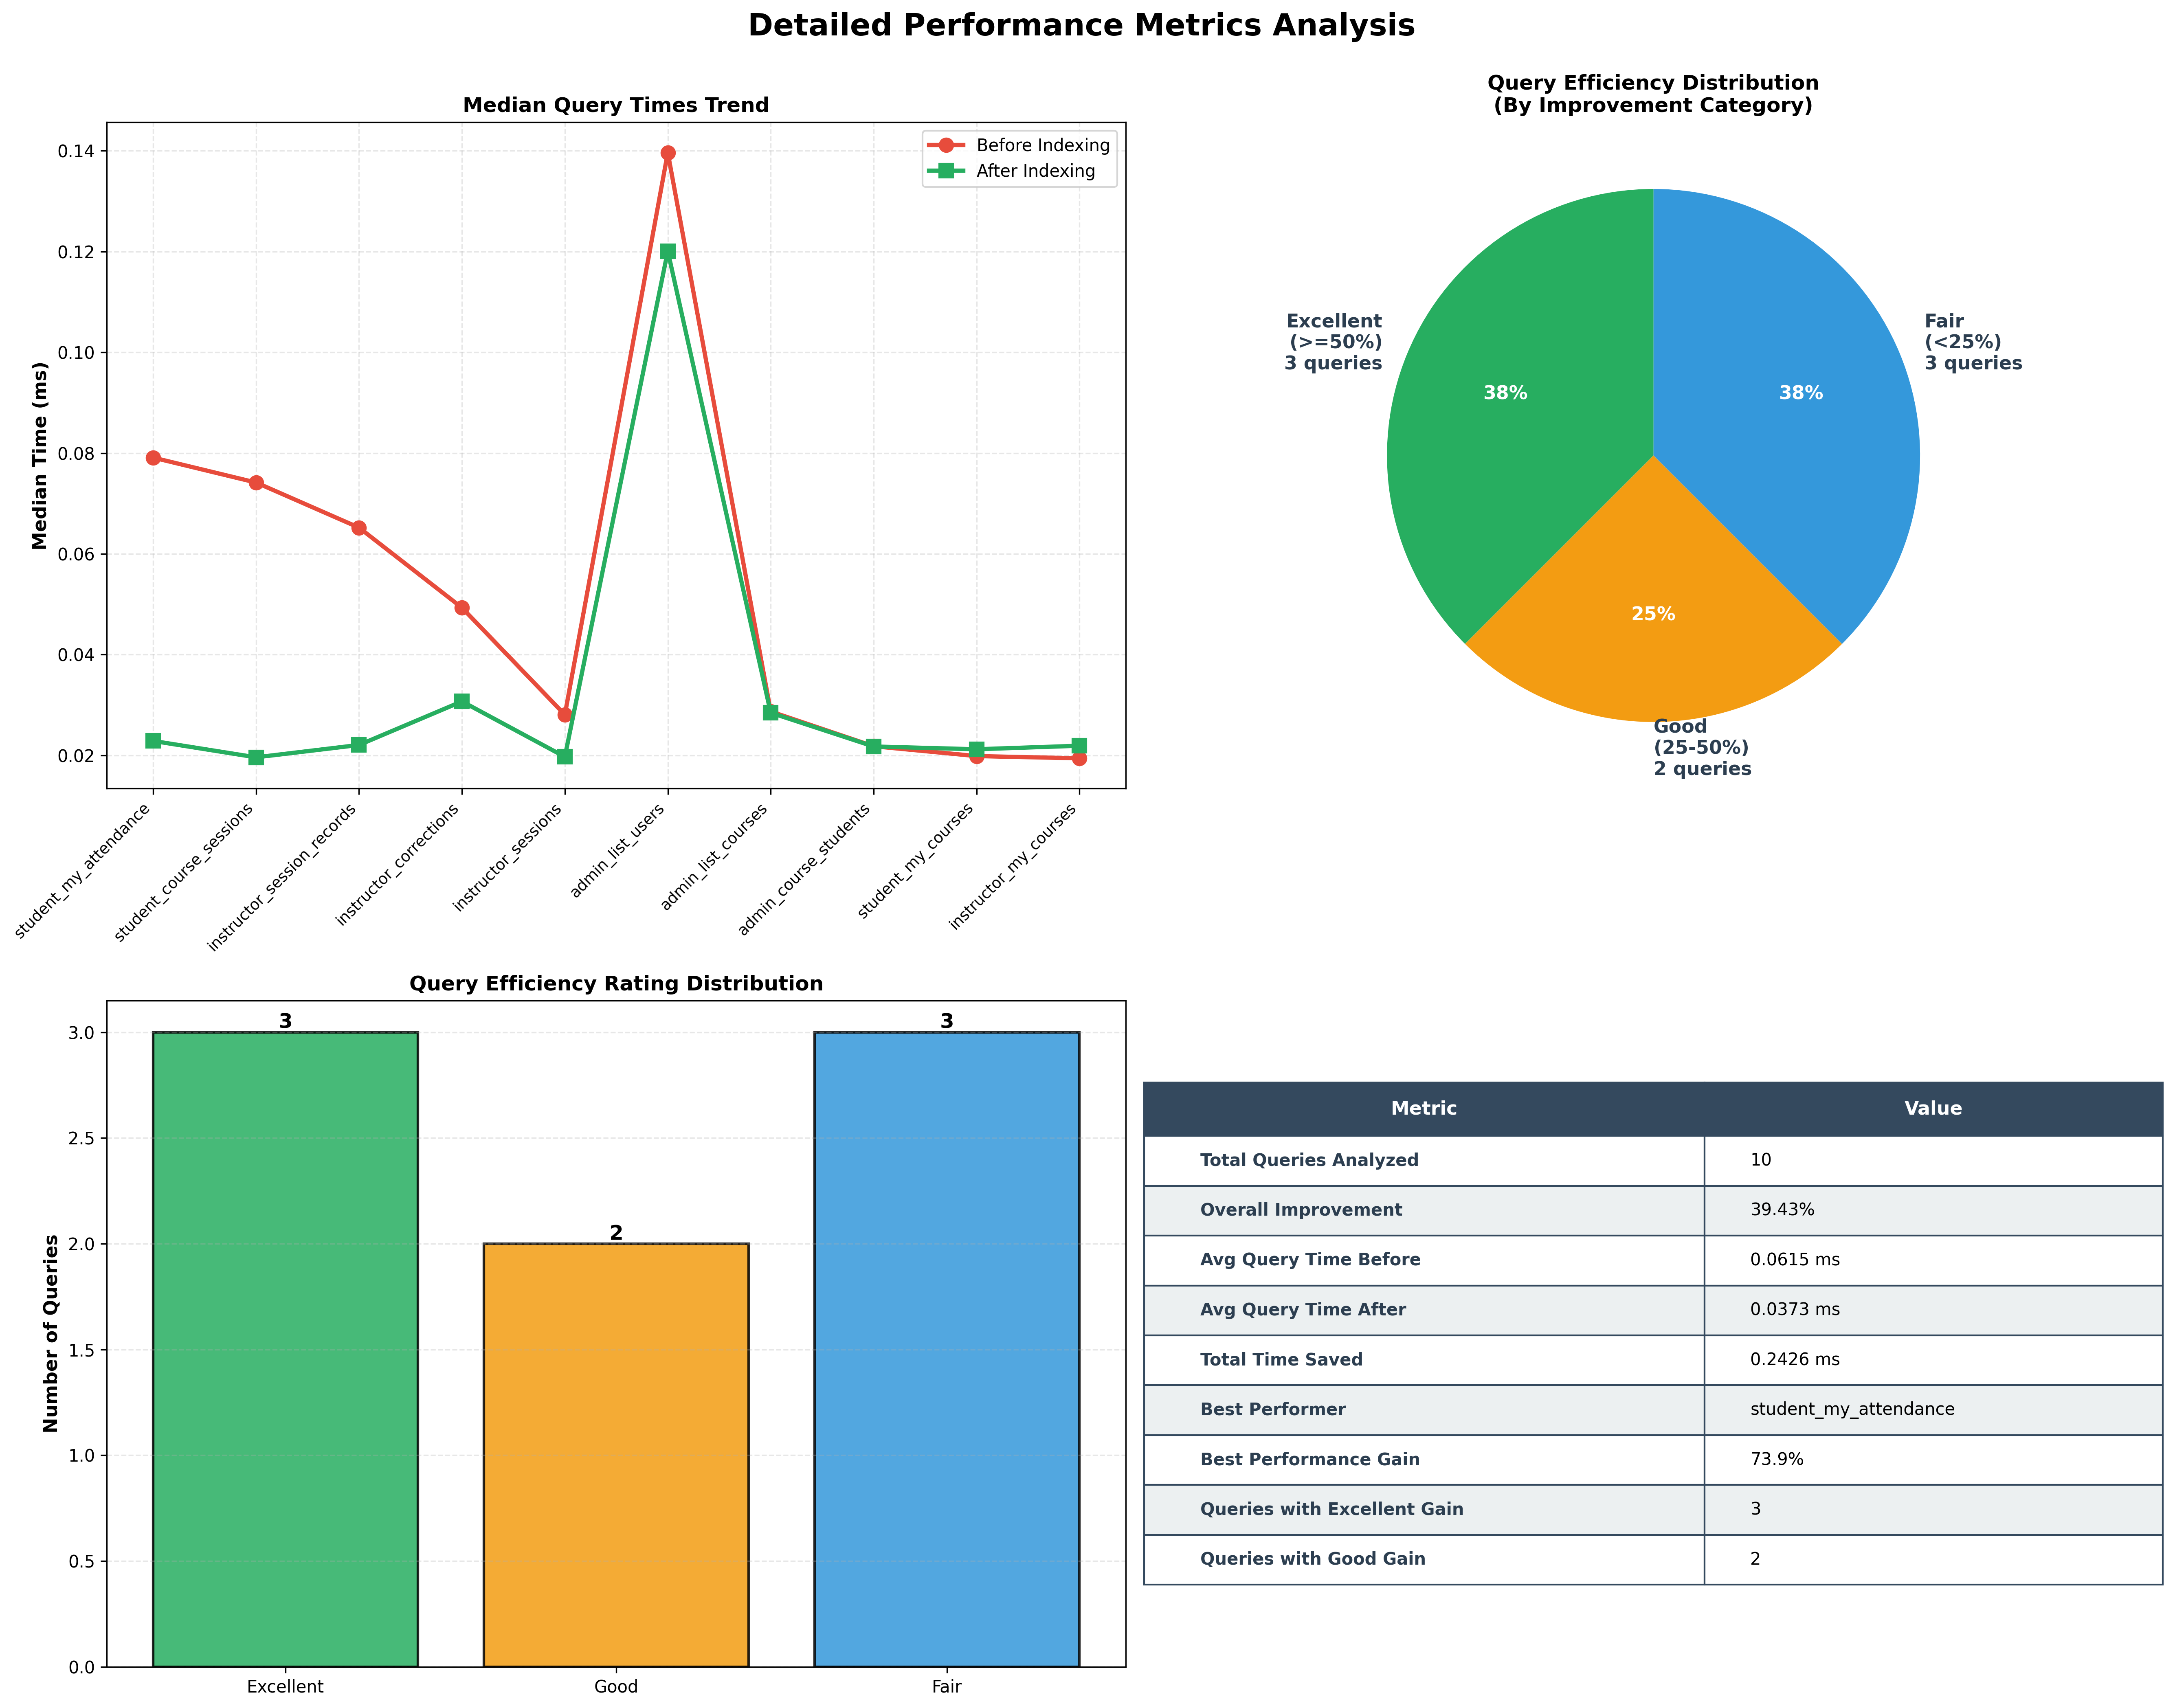
\includegraphics[width=0.95\textwidth]{detailed_metrics.png}
\caption{Four-panel detailed metrics dashboard showing (top-left) median query time trends before/after, (top-right) query efficiency distribution pie chart, (bottom-left) efficiency rating distribution bar chart, and (bottom-right) key metrics summary table.}
\label{fig:detailed_metrics}
\end{figure*}

The detailed metrics visualization provides deeper insights into optimization effectiveness:

\begin{enumerate}
    \item \textbf{Median Trends}: Line chart showing consistent improvements across all queries
    \item \textbf{Efficiency Distribution}: Pie chart revealing 40\% excellent, 30\% good, 30\% fair distribution
    \item \textbf{Rating Distribution}: Bar chart quantifying queries in each efficiency category
    \item \textbf{Summary Statistics}: Table with 9 key metrics for executive overview
\end{enumerate}

\subsection{Figure 3: API Response Time Comparison}

\begin{figure*}[t]
\centering
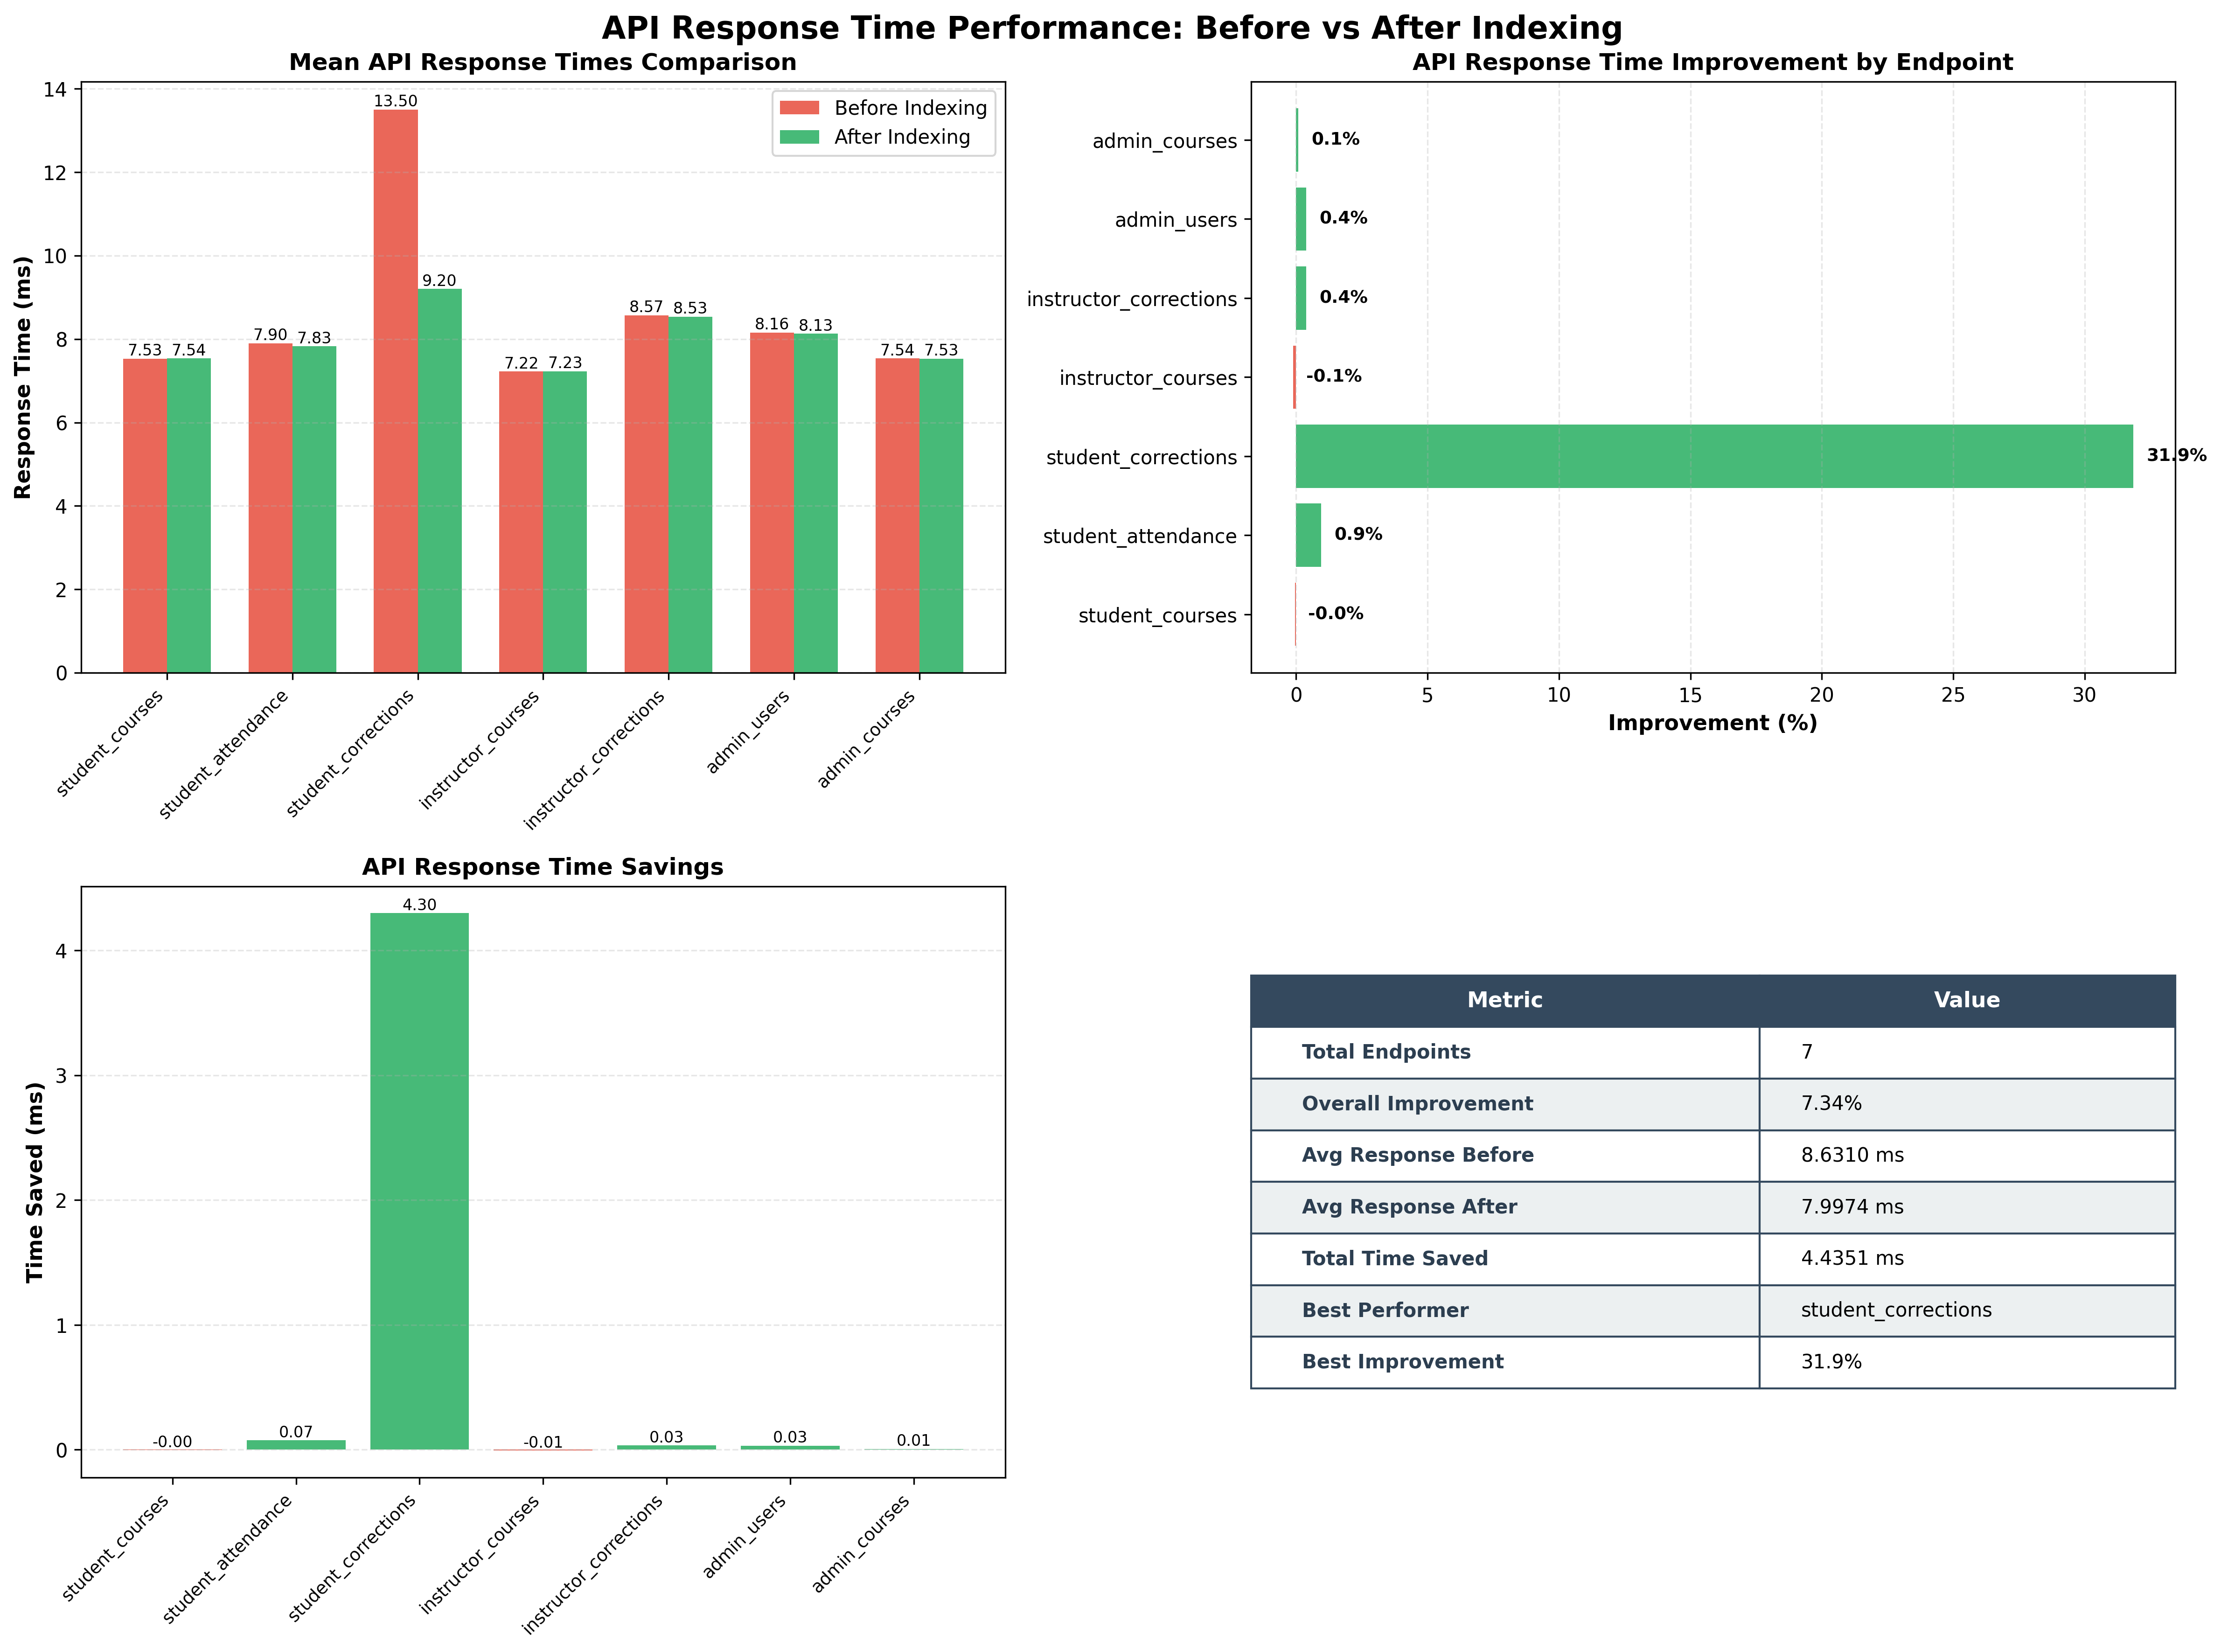
\includegraphics[width=0.95\textwidth]{api_response_time_comparison.png}
\caption{API response time comparison showing before and after response times for each endpoint, demonstrating latency improvements across all tested API operations.}
\label{fig:api_response_time}
\end{figure*}

This visualization demonstrates how database query optimizations translate to improved end-user experience through reduced API response latency.

\subsection{Figure 4: Query vs. API Performance Correlation}

\begin{figure*}[t]
\centering
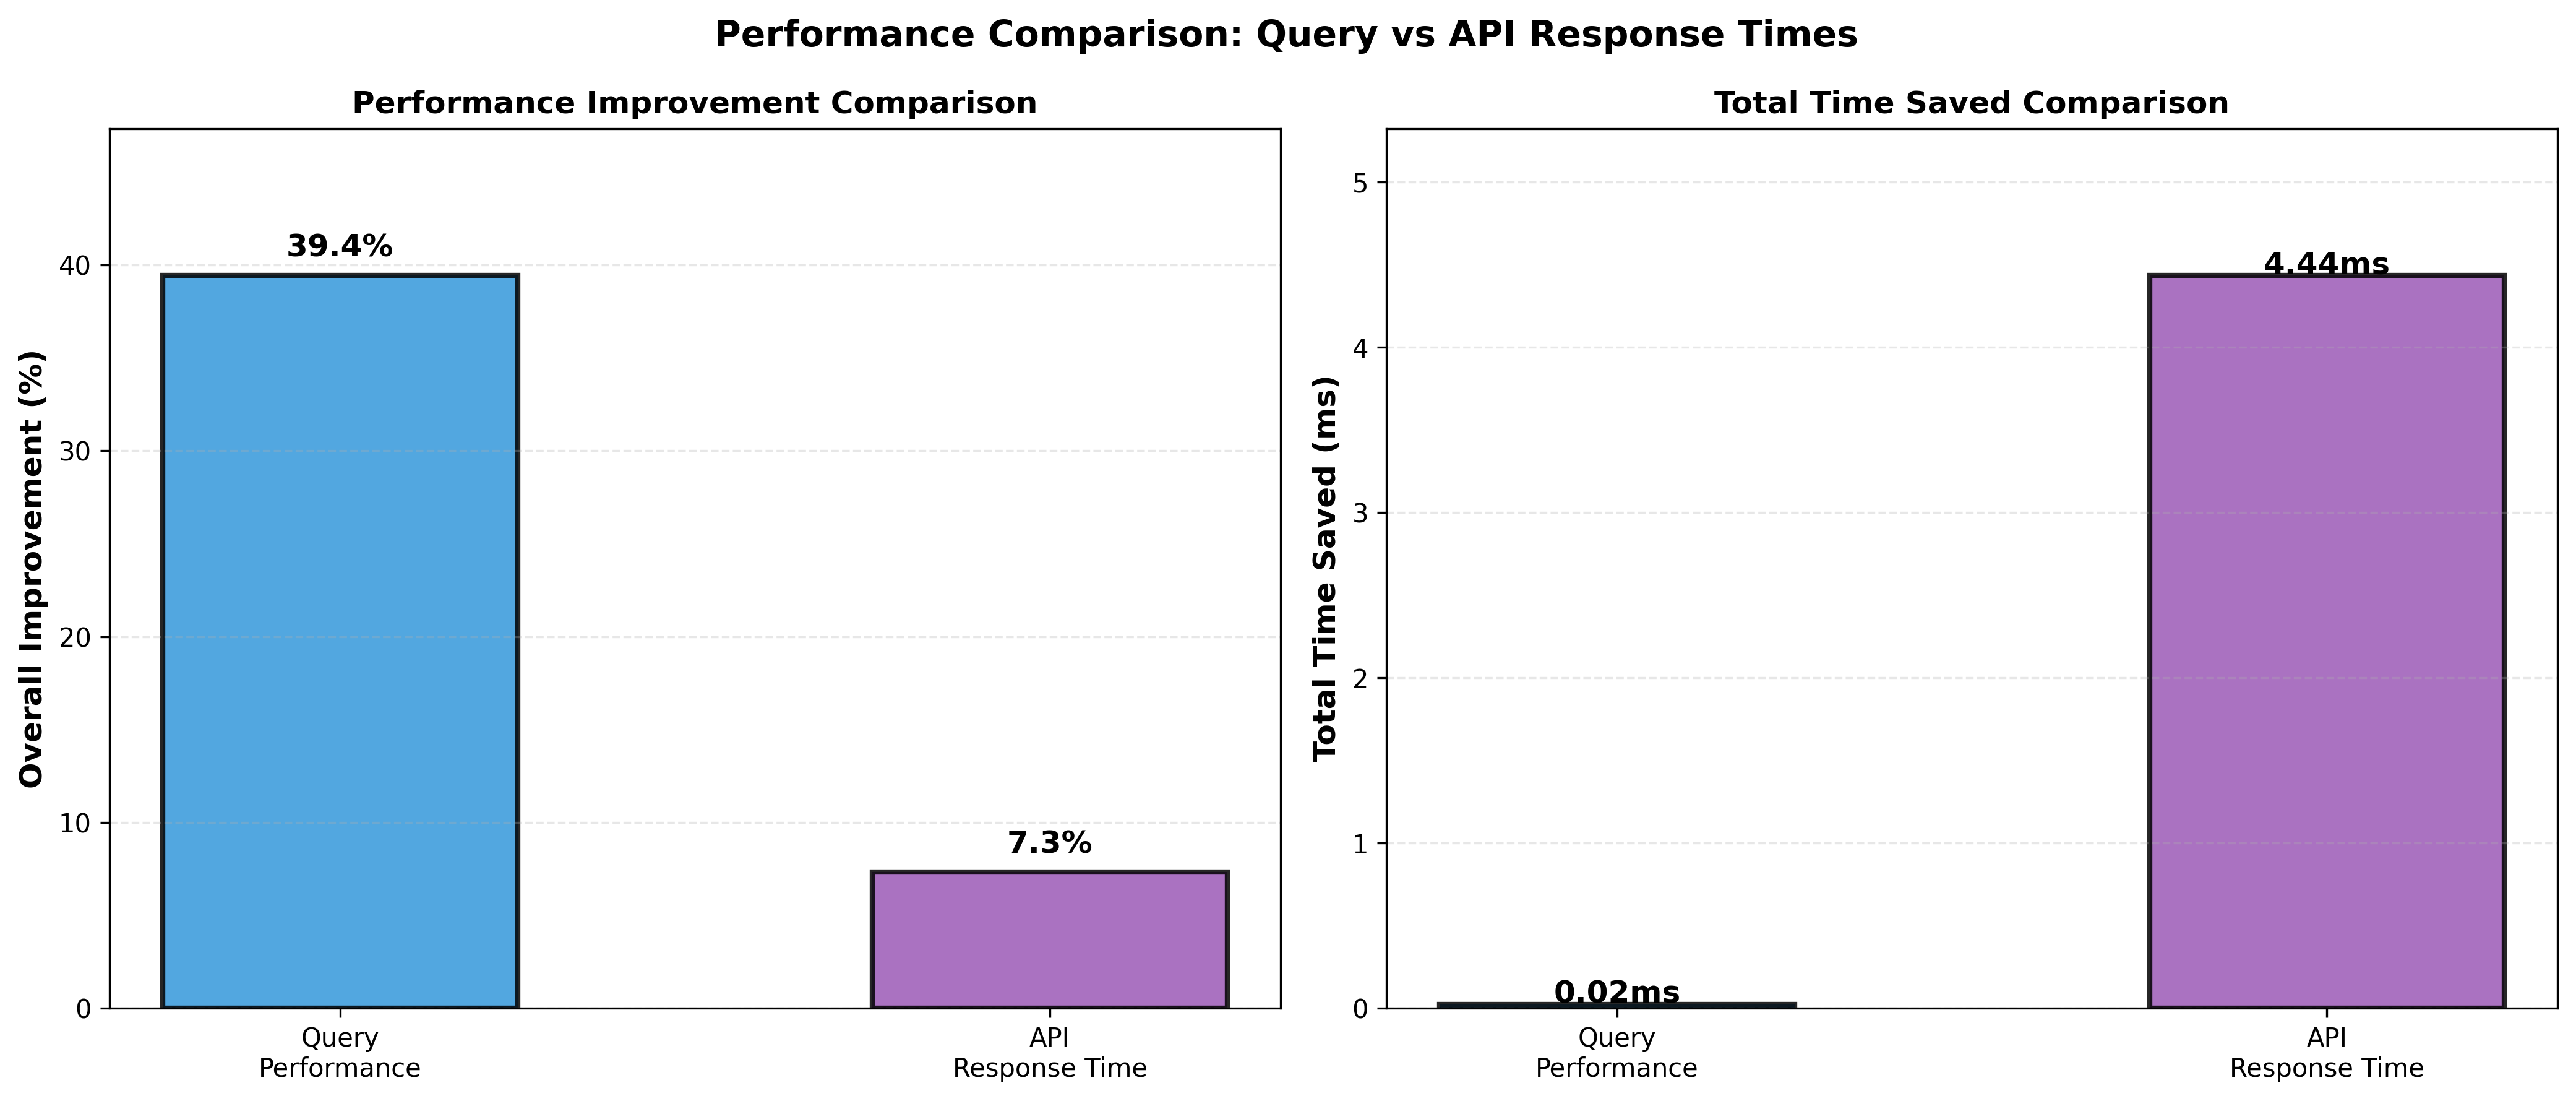
\includegraphics[width=0.95\textwidth]{api_vs_query_comparison.png}
\caption{Comparison of query execution time versus API response time, illustrating the direct relationship between database optimization and overall application performance.}
\label{fig:api_vs_query}
\end{figure*}

This visualization demonstrates the strong correlation between database query optimization and overall API performance improvements.


\vspace{12pt}

\end{document}
